%%%%%%%%%%%%%%%%%%%%%%%%%%%%%%%%%%%%%%%%%
% Stylish Article
% LaTeX Template
% Version 2.2 (2020-10-22)
%
% This template has been downloaded from:
% http://www.LaTeXTemplates.com
%
% Original author:
% Mathias Legrand (legrand.mathias@gmail.com) 
% With extensive modifications by:
% Vel (vel@latextemplates.com)
%
% License:
% CC BY-NC-SA 3.0 (http://creativecommons.org/licenses/by-nc-sa/3.0/)
%
%%%%%%%%%%%%%%%%%%%%%%%%%%%%%%%%%%%%%%%%%

%----------------------------------------------------------------------------------------
%	PACKAGES AND OTHER DOCUMENT CONFIGURATIONS
%----------------------------------------------------------------------------------------

\documentclass[fleqn,10pt]{SelfArx} % Document font size and equations flushed left
\usepackage{float}
\usepackage[english]{babel} % Specify a different language here - english by default
\usepackage[numbers]{natbib}
\usepackage{url}
\usepackage{lipsum} % Required to insert dummy text. To be removed otherwise
\usepackage{tabularx}
\usepackage{tcolorbox}
\usepackage{siunitx}
\tcbuselibrary{xparse}
\usepackage{graphicx} 
\usepackage{caption,subcaption}

\sisetup{
    group-digits=true,
    group-separator={\,},
}
%----------------------------------------------------------------------------------------
%	COLUMNS
%----------------------------------------------------------------------------------------

\setlength{\columnsep}{0.55cm} % Distance between the two columns of text
\setlength{\fboxrule}{0.75pt} % Width of the border around the abstract

%----------------------------------------------------------------------------------------
%	COLORS
%----------------------------------------------------------------------------------------

\definecolor{color1}{RGB}{0,0,90} % Color of the article title and sections
\definecolor{color2}{RGB}{0,20,20} % Color of the boxes behind the abstract and headings

%----------------------------------------------------------------------------------------
%	HYPERLINKS
%----------------------------------------------------------------------------------------

\usepackage{hyperref} % Required for hyperlinks

\hypersetup{
	hidelinks,
	colorlinks,
	breaklinks=true,
	urlcolor=color2,
	citecolor=color1,
	linkcolor=color1,
	bookmarksopen=false,
	pdftitle={Title},
	pdfauthor={Author},
}

%----------------------------------------------------------------------------------------
%	ARTICLE INFORMATION
%----------------------------------------------------------------------------------------

\JournalInfo{Data Scientist Nanodegree} % Journal information
\Archive{Capstone Project} % Additional notes (e.g. copyright, DOI, review/research article)

\PaperTitle{Short Term Stock Price Prediction with Machine Learning} % Article title

\Authors{Lucas Breinlinger\textsuperscript{1}} % Authors
\affiliation{\textsuperscript{1}\textit{Contact: lucas.nm.breinlinger@bmw.com}} % Author affiliation


\Keywords{} % Keywords - if you don't want any simply remove all the text between the curly brackets
\newcommand{\keywordname}{Keywords} % Defines the keywords heading name

%----------------------------------------------------------------------------------------
%	ABSTRACT
%----------------------------------------------------------------------------------------

\Abstract{Accurately predicting stock prices is a highly sought-after mastery. In recent years Long Short Term Memory (LSTM), a type of recurrent neural network, has proven to be highly promising in achieving better predictions. Using a simple LSTM with only 25 neurons already can predict loosely the future stock prices based on the stock prices of the previous 30 days. The refined model with two LSTM layers with 150 neurons and two dense layers is very successful in predicting the future close price.}

%----------------------------------------------------------------------------------------

\begin{document}

\maketitle % Output the title and abstract box

\tableofcontents % Output the contents section

\thispagestyle{empty} % Removes page numbering from the first page

%----------------------------------------------------------------------------------------
%	ARTICLE CONTENTS
%----------------------------------------------------------------------------------------

\section{Project Definition} % The \section*{} command stops section numbering

The accurate forecast of stock prices, traded on an exchange, is inarguably one of the most challenging topics in the field of asset pricing. The stock market is described as an unpredictable, dynamic and non-linear construct. Predicting the prices of its stocks is an ambitious undertaking and depends on many variables including but not limited to the global economy, the company's metrics and local and global political situation. 
\\
\\
Historically there are two main prediction methods. The fundamental analysis which is a qualitative analysis of the company is interested in finding the true value of a stock and comparing it to the actual traded value. The evaluator utilizes several performance criteria e.g. the P/E ratio to truly assess the underlying stock. Secondly, the technical analysis, which is solely based on the past price of the stock e.g. in form of closing or opening prices as time-series. It is rather a short-term prediction using factors like the Moving Average (MA) or the Exponential Moving Average (EMA). Its basic assumption is that every significant information about the stock is already considered in the stock price \cite{prediction}.
\\
\\
The fast computational development has led to the point that Machine learning techniques have a significant application in financial problems. The use of artificial neural networks has found more and its way into the field of stock price prediction. Here a recurrent neural network (RNN) has been found very proven, more precisely the Long Short Term Memory (LSTM). Its advantage is being
able to process entire sequences of data rather than only one single data point. It has proven to be very practical with time series data such as our historical stock prices. 
\\
In this project, I create an application that is going to predict the \textbf{closing price} of any given stock on which it is trained. For the sake of convenience, this report only considers the stock price prediction of the \textbf{Apple} Inc. (\textit{\$AAPL}) stock.
\\
A train-test cycle is used to test the accuracy of the prediction. The root mean squared error (\ref{eq.rmse}) is used to measure the accuracy of the model:
\begin{equation}
RMSE = \sqrt{\dfrac{\Sigma_{i}(\hat{y}_i-y_i)}{N}} 
\label{eq.rmse}
\end{equation}
where $\hat{y}_i$ is the prediction of the $i-th$ stock price $y_i$ and $N$ is the total number of predicted stock prices.

In the next section, I will analyze the data and give some insights about the data. Afterwords I will explain the methodology and discuss the results. In the end, I give an outlook for further developments and improvements.

%------------------------------------------------

\section{Data Analysis}

\begin{table*}[hbt]
	\caption{First lines of \textit{Apple Inc.} stock prices dataset}
	\centering
\begin{tabular}{lllrrrr S[table-auto-round,table-format=9.0] rr}
\toprule
Ticker &       Name &       Date &  Open &  High &   Low &  Close &       {Volume} &  Dividends &  Stock Splits \\
\midrule
  AAPL & Apple Inc. & 2012-07-19 & 18.77 & 18.90 & 18.61 &  18.87 & 436861600.00 &       0 &          0 \\
  AAPL & Apple Inc. & 2012-07-20 & 18.83 & 18.87 & 18.54 &  18.56 & 397471200.00 &       0 &          0 \\
  AAPL & Apple Inc. & 2012-07-23 & 18.25 & 18.61 & 18.05 &  18.54 & 487975600.00 &       0 &          0 \\
  AAPL & Apple Inc. & 2012-07-24 & 18.65 & 18.72 & 18.38 &  18.45 & 565132400.00 &       0 &          0 \\
  AAPL & Apple Inc. & 2012-07-25 & 17.64 & 17.84 & 17.51 &  17.66 & 877312800.00 &       0 &          0 \\
\bottomrule
\end{tabular}
	\label{tab:df.head}
\end{table*}

\begin{table*}[hbt]
	\caption{Statistics of the Apple stock prices. Which represent our used features}
	\centering
\begin{tabular}{lS[table-auto-round,table-format=9.1] S[table-auto-round,table-format=9.1] S[table-auto-round,table-format=9.1] S[table-auto-round,table-format=9.1]S[table-auto-round,scientific-notation = engineering, table-format=-1.1e-1]  S[table-auto-round,table-format=9.0]}
\toprule
{} &         {Open} &         {High} &          {Low}&        {Close}              \\
\midrule
count &  2514.000000 &  2514.000000 &  2514.000000 &  2514.000000  \\
mean  &    54.976304 &    55.586809 &    54.385991 &    55.010195 \\
std   &    45.998891 &    46.593796 &    45.425948 &    46.036470  \\
min   &    12.090742 &    12.453181 &    12.001301 &    12.170523  \\
25\%   &    22.846671 &    23.103172 &    22.672594 &    22.848148 \\
50\%   &    36.503730 &    36.712400 &    36.239020 &    36.499804  \\
75\%   &    66.667990 &    68.501637 &    65.989975 &    67.521479  \\
max   &   182.630005 &   182.940002 &   179.119995 &   182.009995  \\
\bottomrule
\end{tabular}
	\label{tab:df.statistrics}
\end{table*}


The dataset was collected with the help of \tcboxverb{yfinance} python plugin. In my case, it is replacing the not working Yahoo Finance API. The collected data frame contains
\begin{itemize}[noitemsep] % [noitemsep] removes whitespace between the items for a compact look
	\item \num{1108837} rows
	\item $10$ columns
	\item price information for $457$ unique stocks
	\item Data of the last 10 years (including 17/07/2022)
\end{itemize} and was collected on 18/07/2022. I use a list of 457 randomly selected stock tickers to generate the dataset. 

The structure and the first 5 lines of the table filtered for \textit{Apple Inc.} are displayed in table \ref{tab:df.head}. For each day and each stock (denoted by its ticker (\textit{Ticker}) and company name (\textit{Name}) the dataset contains the price of the stock in dollar 
when opening the market (\textit{Open}), closing the market (\textit{Close}). Furthermore there the days lowest (\textit{Low}) and highest 
intra-day price (\textit{High} is available, as well as the daily traded volume (\textit{Volume}).


Looking at the \textit{Apple Inc.} stock there are 2514 columns regarding the apple stock with a minimum closing price of $12.17$ and a maximum closing price of $182.01$. There are no missing values (see table \ref{tab:df.statistrics}) in the dataset, and the date and value columns are correctly set as a datetime respectively float columns. In table \ref{tab:df.statistrics}, the statistics of the distinctive variables are shown.

\begin{figure}[ht]\centering
	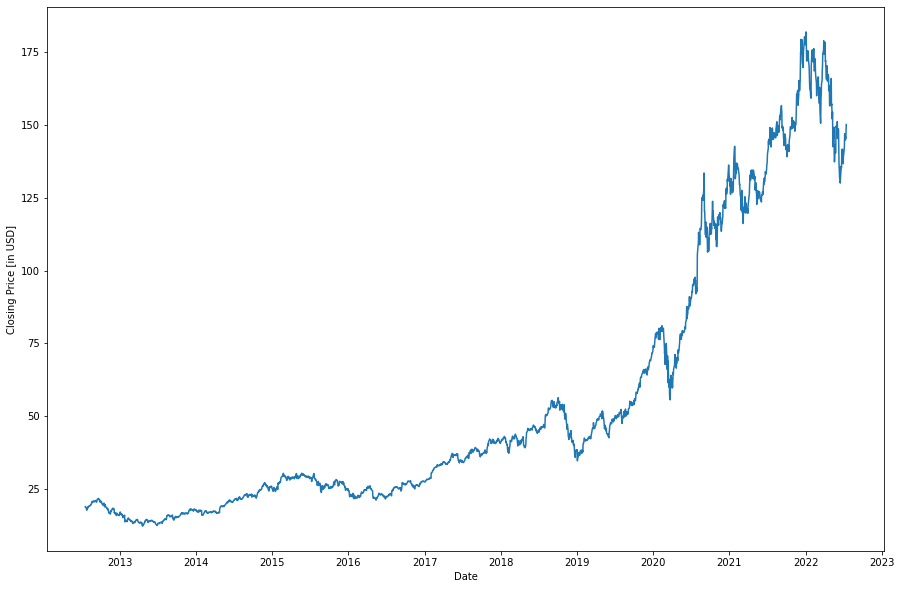
\includegraphics[width=\linewidth]{closing}
	\caption{Closing price of the \textit{Apple Inc.} in the last 10 years.}
	\label{fig:results}
\end{figure}

In figure \ref{fig:results}, the highly volatile closing price of the stock is shown for its last 10 years. In recent years the stock prices have increased roughly sevenfold. In the next section, I am going to explain the methodology, followed by a chapter discussing the results.




%------------------------------------------------

\section{Methodology}

\begin{figure*}[htb]\centering % Using \begin{figure*} makes the figure take up the entire width of the page
	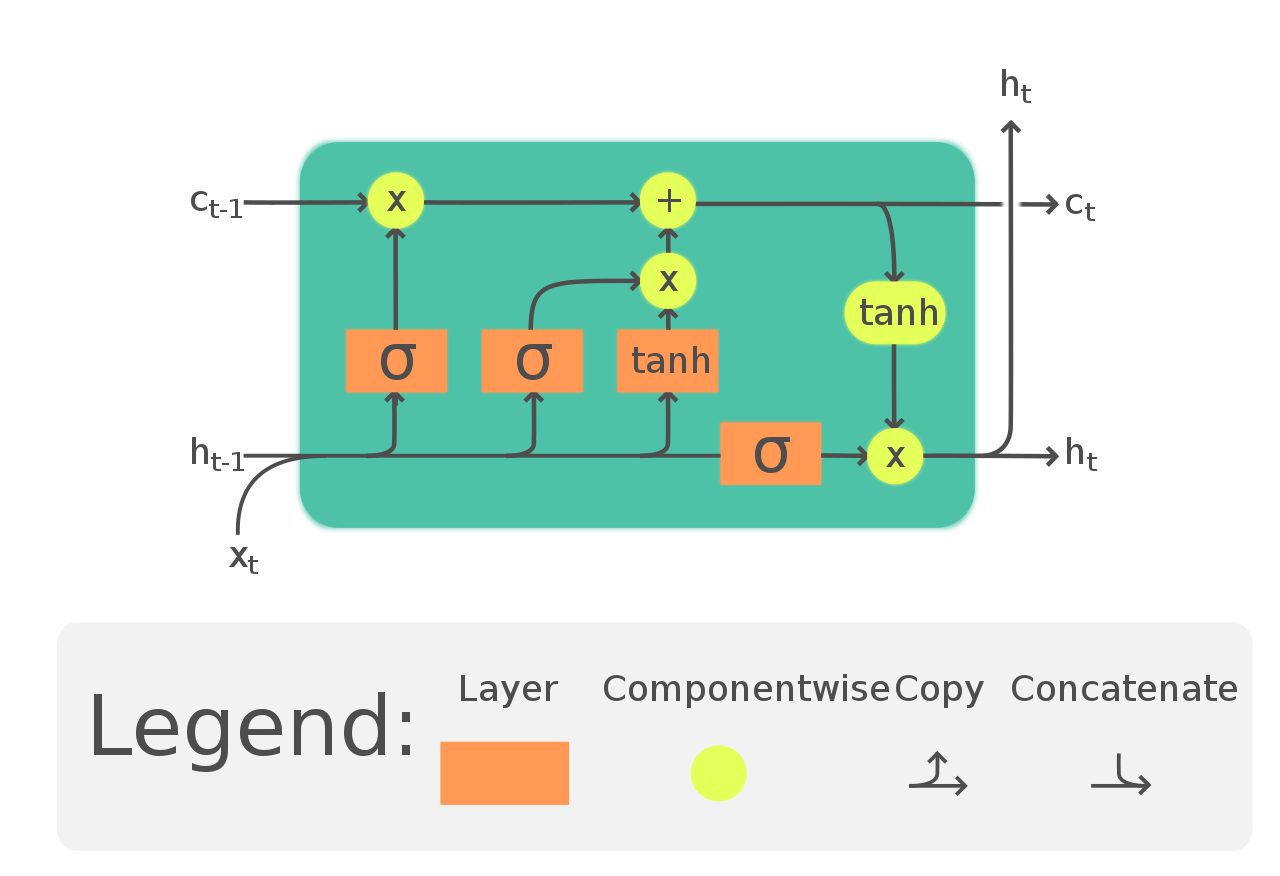
\includegraphics[width=0.8\linewidth]{LSTM}
	\caption{The reccurent cell of a LSTM network \cite{LSTM}.}
	\label{fig:lstm.network}
\end{figure*}

Here, I am using a Recurrent Neural Network for the stock price prediction. More specifically a Long Short Term Memory Network is used to build the model. These networks are capable of learning long-term dependencies and are commonly used for handling and forecasting time-series data. In figure \ref{fig:lstm.network}, a recurrent cell of a LSTM network is shown. Each cell consists of three gates, an input gate, an output gate and a forget gate. \cite{LSTMexplained}

Those cells are linked together to a chain, where each cell looks at the input gate at the previous hidden state $h_{t-1}$, the current input $x_t$, and the previous cell state $c_{t-1}$. The forget cell is the first part where $h_{t-1}$ and $x_t$ are passed through the sigmoid activation function and pointwise multiplied with the cell state $c_{t-1}$. The input gates combine a sigmoid and tanh layer, here it is decided which parts are going to be updated. Multiplying both layers determines which information is used to update the cell state by pointwise adding it to the output of the forget gate, resulting in the final $c_t$.
In the output gate, the same input ($h_{t-1}$ and $x_t$) is passed through a sigmoid function and finally multiplied with the current cell state $c_t$, yielding the final output the hidden state $h_t$. \cite{LSTMexplained1}

For the LSTM to work properly, the stock closing prices have to be normalized. This will help our model to converge faster and be more stable. Furthermore, when using the scaler on more than one input feature with different scales all features will contribute equally to the fitting and there will be no bias due to a different scaling \cite{normalize}. I am using the MinMaxScaler (\ref{eq.minmax}) of sci-kit learn.
\begin{equation}
x_{i,scaled}=\dfrac{x_i-min(x)}{max(x)-min(x)}
\label{eq.minmax}
\end{equation}

Here, I am trying to predict future stock prices $y_t$ (target) with the help of the previous $n$ stock prices. For example, I am predicting the stock price from day 11 using day 1 to 10 as my features, for day 12, using day 2-11 and so on. In order to do this, I defined a splitting function that generates a data sample consisting of $n$ samples (the previous stock prices) and the target value $n + 1$. $n$ is denoting the size of my window which I am using to predict the prices. This function is applied to my previously scaled stock prices. 

Finally, I split this data set into a training and a test set, since we are dealing with a time-series we cannot randomly select the samples, rather I split the sample at some point. In my experiment, I am using $80\%$ as a training set and the remaining $20\%$ as my test set. Using the predicted stock price $\hat{y}_i$ and the real stock price $y_t$ of the test set the RMSE can be easily calculated using eq. \ref{eq.rmse}.

\begin{table}[hbt]
	\caption{Overview of the model parameters.}
	\centering
	\scalebox{0.8}{
\begin{tabular}{lcccccc}
\hline
Model & LSTM 1 & LSTM 2 & Dense 1 & Dense 2 & Epoch & $n$ \\ 
\hline 
simple & 10 & - & 1 & - & 1 & 30 \\ 

refined 1 & 10 & 10 & 25 & 1 & 1 & 30 \\ 

refined 2 & 50 & 50 & 25 & 1 & 1 & 30 \\ 

refined 3 & 150 & 150 & 25 & 1 & 5 & 30 \\
\end{tabular}}

\label{table.model} 
\end{table}

The first \textbf{simple model} I build, consisted of a single LSTM layer with 10 neurons and a dense Layer with 1 neuron. The dense layer is needed to get the dimensionality of the output of the LSTM $h_t$ back to a 1D output. I am using the previous thirty close prices ($n=30$) as my input $x_t$.

My refined model is a deeper neural network since the relations between stock prices are quite complicated. Thus, I added an LSTM layer and a second dense layer with 25 neurons. The refined model is run with different parameters, the first run is 10 neurons for both LSTM layers, the next run is 50 neurons for both layers and in my last model, I am using 150 neurons and 5 epochs. All the time $n$ is kept at $30$ days.

In table \ref{table.model} the model parameters are shown in an overview. In the next section, I will discuss the results of these models.


\section{Results}

\begin{table}[H]
	\caption{The resulting $RMSE$ of the four models.}
	\centering
	\begin{tabular}{cr}
	\hline 
	Model & $RMSE$ \\ 
	\hline 
	simple & 37.83 \\ 
	refined 1 & 28.34 \\ 
	refined 2 & 9.59 \\ 
	refined 3 & 3.74 \\ 
	\hline 
	\end{tabular} 
	\label{tab:rsme}
\end{table}

As expected the $RMSE$ for the refined model is smaller than for the simple model. Furthermore, refined model 3 with 150 neurons per LSTM and 5 epochs also performed better than refined models 1 and 2 with fewer neurons and only one epoch. 

For comparison see the values for all four models in table \ref{tab:rsme}.n figure \ref{fig:results} the predicted stock prices for all models are plotted versus the actual stock price. Furthermore figure \ref{fig:results} is a detailed view of the stock price prediction for the last 60 days. 

As one can see in the detailed graphics for each model, the more complicated the model, the better the prediction. The poor performance of the simple model can be seen in figure \ref{fig:simple} and \ref{fig:simple_zoom}. The prediction follows loosely the real price, however, it is much higher than the real price.  The refined model 1 already performs slightly better than the simple model (compare RMSE) and figure \ref{fig:refined1} and \ref{fig:refined_zoom1}, but also fails to make an accurate prediction.

A huge leap in prediction accuracy is made when the number of neurons is increased from refined model 1 to refined model 2. This accuracy can even be improved by tripling the number of neurons and going through the dataset 5 times (epochs). The predicted price follows closely the actual price, see \ref{fig:refined_zoom2}. 

The refined model 3 is the most accurate of my models. It has the lowest RMSE and in figure \ref{fig:refined_zoom3} it is visible that it follows closely the actual price.





\begin{figure*}[htb]
    \centering % <-- added
\begin{subfigure}{0.85\columnwidth}
	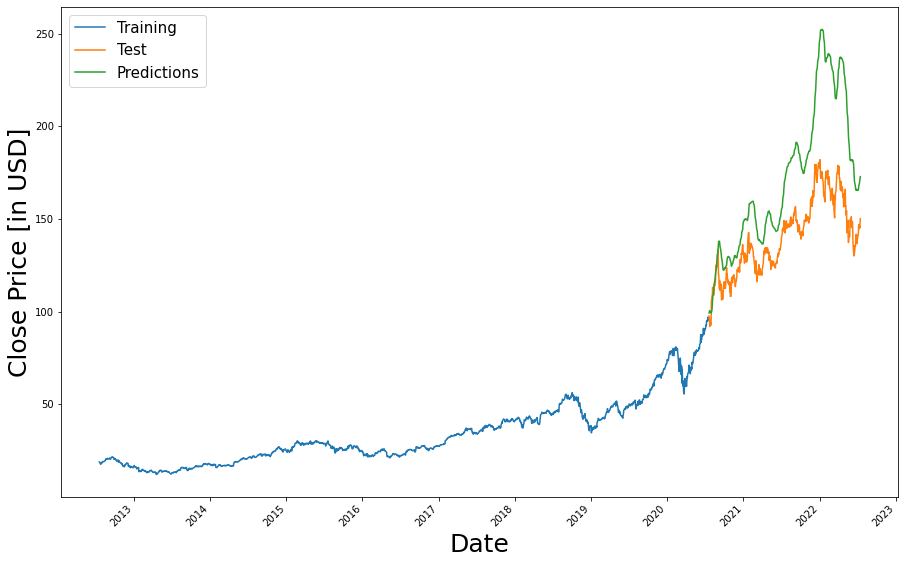
\includegraphics[width=\columnwidth]{simple_model}
	\caption{The prediction close price of the simple model versus the real close price.}
	\label{fig:simple}
\end{subfigure}\hfil % <-- added
\begin{subfigure}{0.85\columnwidth}
	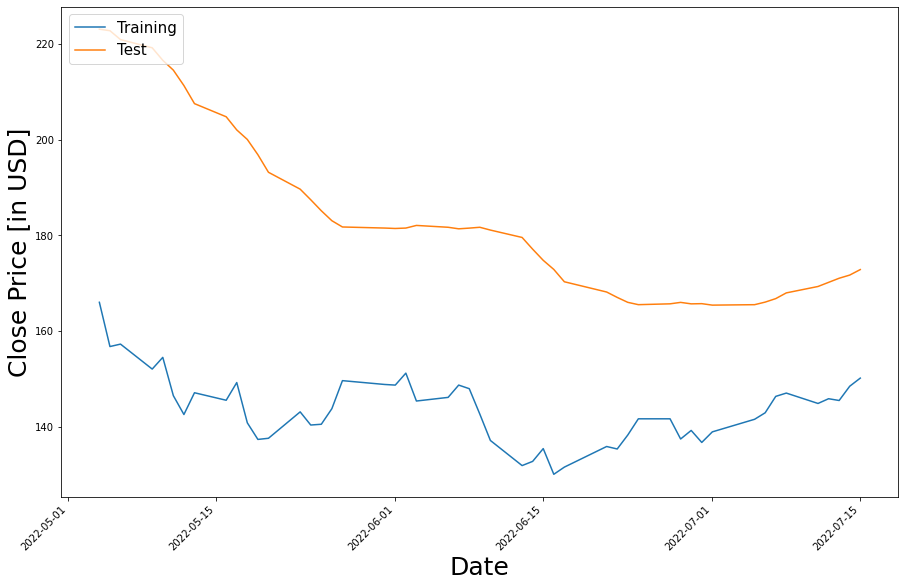
\includegraphics[width=\columnwidth]{simple_model_zoom}
	\caption{The prediction close price for the last 60 days of the simple model versus the real close price.}
	\label{fig:simple_zoom}
\end{subfigure}
\begin{subfigure}{0.85\columnwidth}
	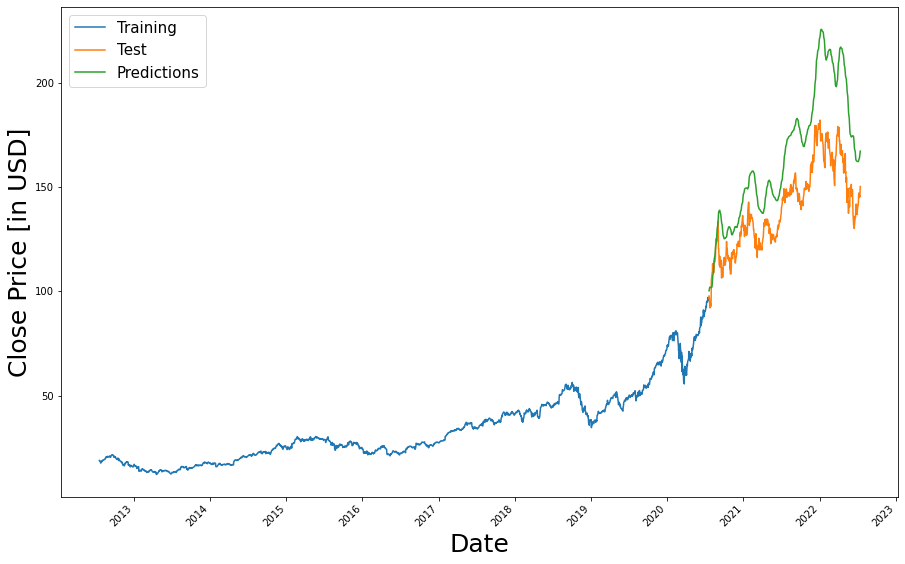
\includegraphics[width=\columnwidth]{refined}
	\caption{The prediction close price of the refined model 1 versus the real close price.}
	\label{fig:refined1}
\end{subfigure}\hfil % <-- added
\begin{subfigure}{0.85\columnwidth}
	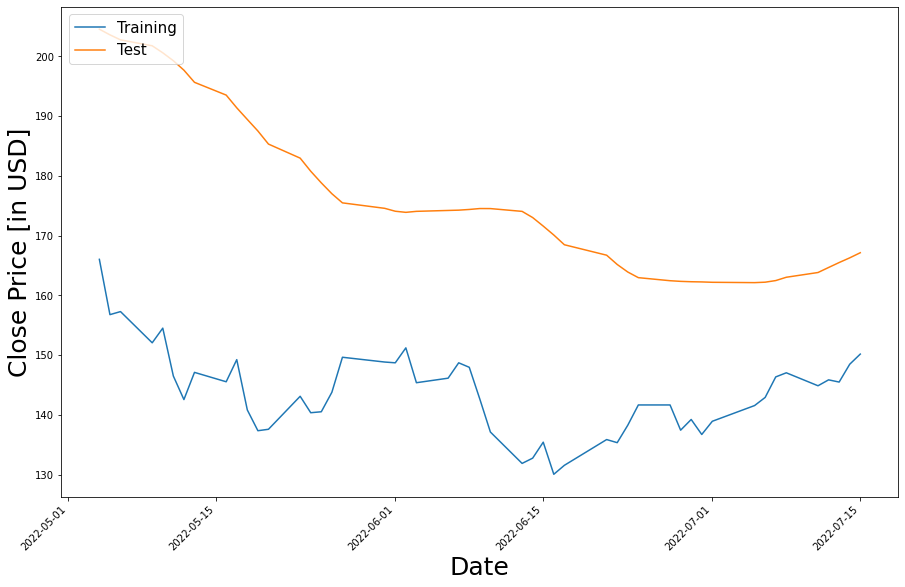
\includegraphics[width=\columnwidth]{refined_zoom}
	\caption{The prediction close price for the last 60 days of the refined model 1 versus the real close price.}
	\label{fig:refined_zoom1}
\end{subfigure}\hfil
\begin{subfigure}{0.85\columnwidth}
	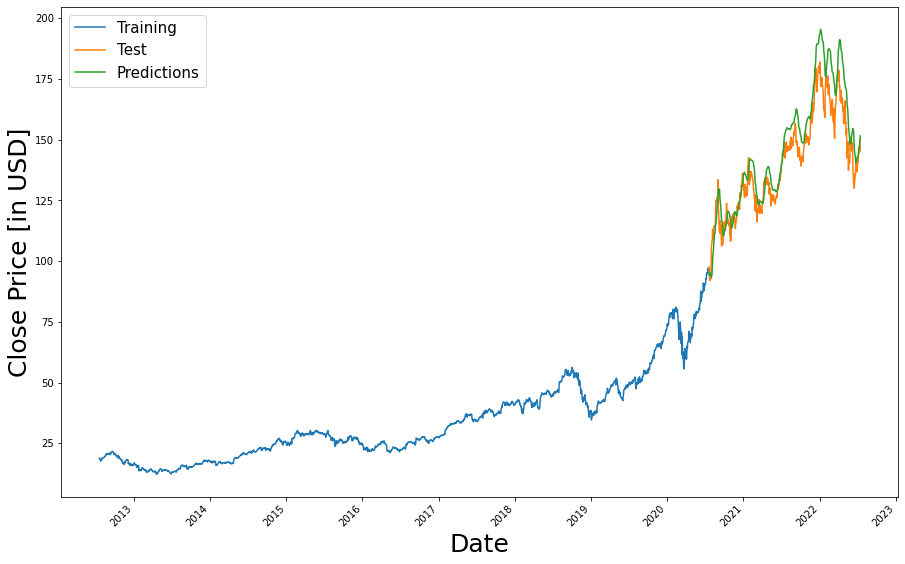
\includegraphics[width=\columnwidth]{refined2}
	\caption{The prediction close price of the refined model 2 versus the real close price.}
	\label{fig:refined2}
\end{subfigure}\hfil % <-- added
\begin{subfigure}{0.85\columnwidth}
	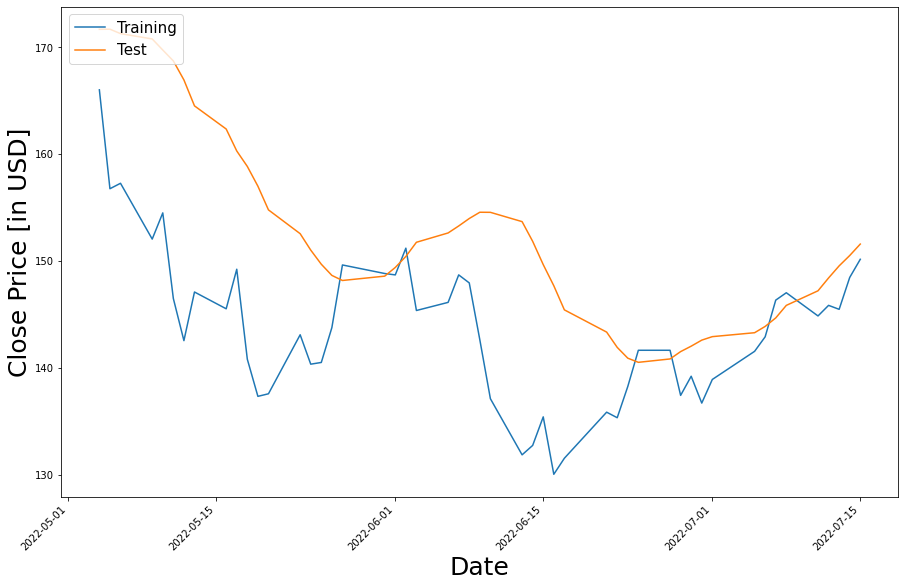
\includegraphics[width=\columnwidth]{refined_zoom2}
	\caption{The prediction close price for the last 60 days of the refined model 2 versus the real close price.}
	\label{fig:refined_zoom2}
\end{subfigure}\hfil
\medskip
\begin{subfigure}{0.85\columnwidth}
	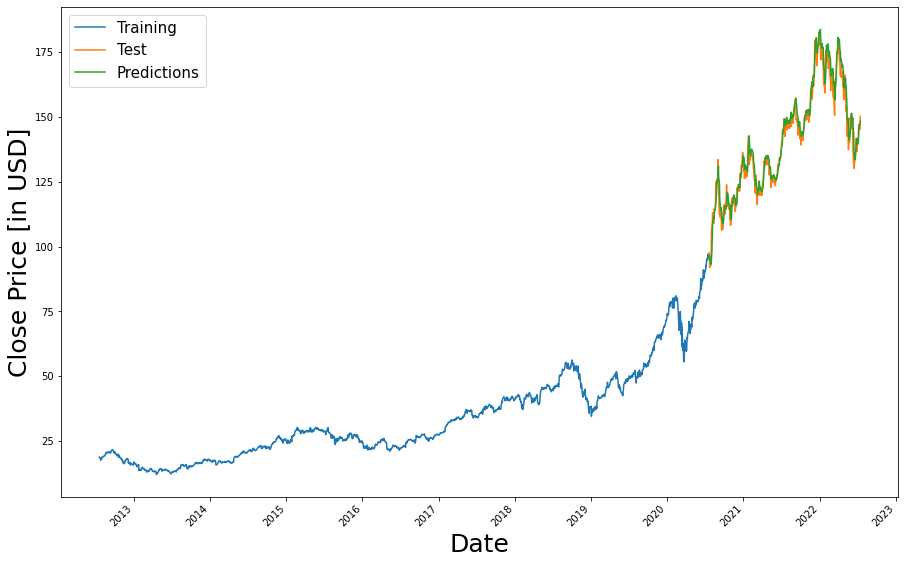
\includegraphics[width=\columnwidth]{refined3}
	\caption{The prediction close price of the refined model 3 versus the real close price.}
	\label{fig:refined3}
	\end{subfigure}\hfil% <-- added
\begin{subfigure}{0.85\columnwidth}
	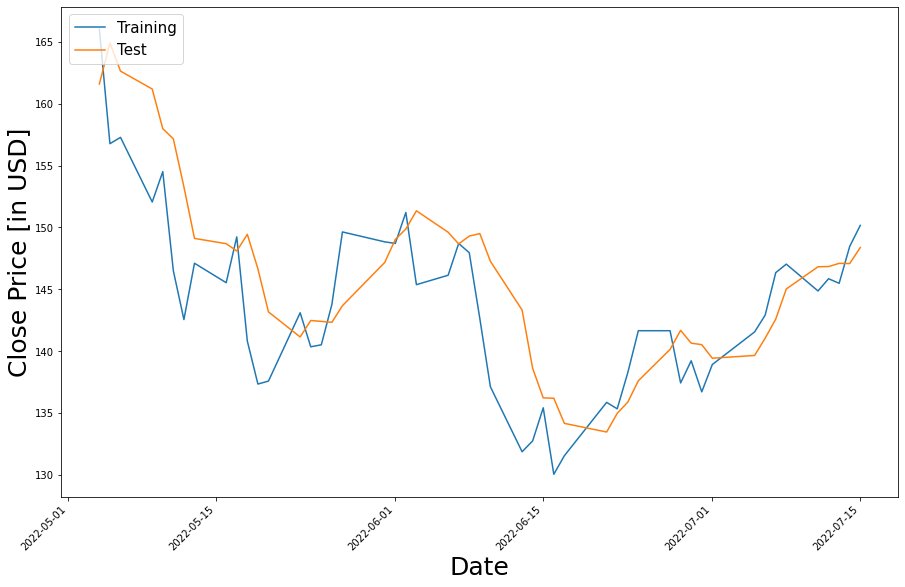
\includegraphics[width=\columnwidth]{refined_zoom3}
	\caption{The prediction close price for the last 60 days of the refined model 3 versus the real close price.}
	\label{fig:refined_zoom3}
	\end{subfigure}
	\label{fig.results}
	\caption{The resulting stock price prediction for all models vs. the actual stock price.}
\end{figure*}



\section{Conclusion}
In this paper, I looked at the problem of forecasting accurately stock prices. In the beginning, I give an overview of why this topic matters so much for the financial world. Additionally, I present some real-life data on the stock prices of Apple stock and some data insights before explaining the methodology. Stock prices can be treated as time-series data, thus LSTM neural networks are predestinated as a suitable algorithm for predicting stock prices. The simple model is falling quite short in predicting the stock prices, however, my most complicated model is roughly 11 times better than the simple one. 

Even though the model is quite good at predicting stock prices, in a real-life scenario it probably will perform poorly due to unforeseen and disruptive events (e.g. COVID19 or Ukraine War).

For future research, I will try and compare different machine learning algorithms and compare their performance with the LSMT. Furthermore one could try to play with the parameters, and layers in my current network to make even better predictions of the future stock price. Also, I will use different stocks and see if the performance of the models is going to change.




%------------------------------------------------



%----------------------------------------------------------------------------------------
%	REFERENCE LIST
%----------------------------------------------------------------------------------------

\phantomsection
\addcontentsline{toc}{section}{References} % Adds this section to the table of contents
\bibliographystyle{unsrt}
\bibliography{sample.bib}

%----------------------------------------------------------------------------------------

\end{document}